\documentclass[tikz,border=6pt]{standalone}
\usepackage{tikz}
\usetikzlibrary{arrows.meta,patterns,decorations.pathreplacing,calc}

\definecolor{kmblue}{RGB}{0,56,116}
\definecolor{kmgold}{RGB}{160,120,0}
\definecolor{rtgreen}{RGB}{30,130,60}
\definecolor{apcol}{RGB}{180,40,40}
\definecolor{isrcol}{RGB}{100,60,160}
\definecolor{taskcol}{RGB}{0,110,160}

\begin{document}
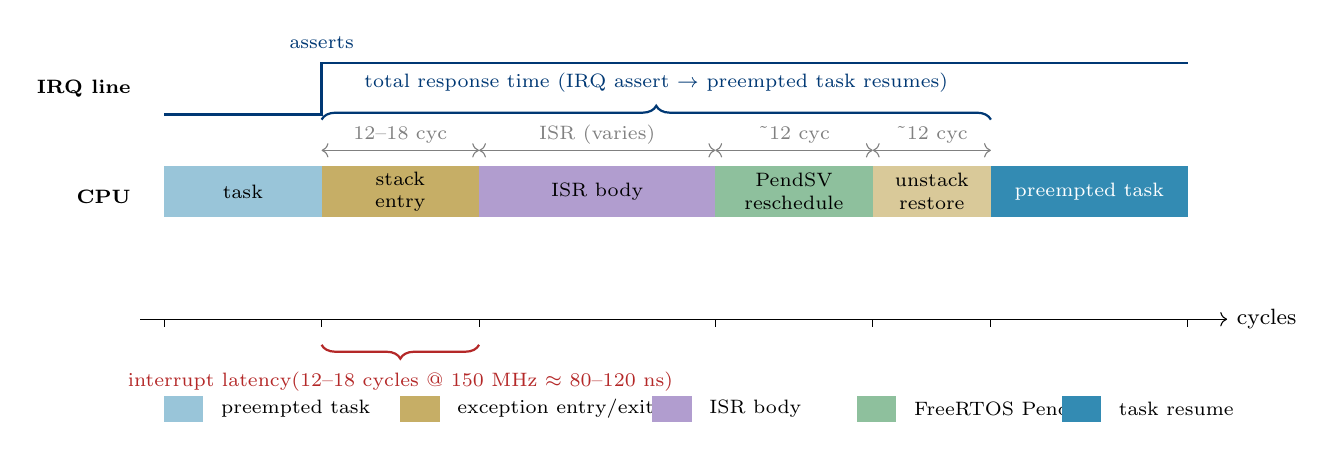
\begin{tikzpicture}[x=1.0cm, y=0.65cm, font=\small]

% ---- Time axis ----
\draw[->] (-0.3,0) -- (13.5,0) node[right]{\footnotesize cycles};

% ---- IRQ signal row (y=4) ----
\node[left, font=\scriptsize\bfseries] at (-0.3,4.5){IRQ line};
\draw[kmblue,thick] (0,4) -- (2,4) -- (2,5) -- (13,5);
\node[font=\scriptsize,kmblue] at (2,5.4){asserts};

% ---- CPU activity row (y=2) ----
\node[left, font=\scriptsize\bfseries] at (-0.3,2.4){CPU};

% Task running before IRQ
\fill[taskcol!40] (0,2) rectangle (2,3);
\node[font=\scriptsize] at (1,2.5){task};

% Tail-chaining / interrupt acceptance (2 cycles approx on M33 if no ISR running)
% Exception entry / stacking: ~12 cycles on M33
\fill[kmgold!60] (2,2) rectangle (4,3);
\node[font=\scriptsize, align=center] at (3,2.5){stack\\entry};

% ISR executes
\fill[isrcol!50] (4,2) rectangle (7,3);
\node[font=\scriptsize] at (5.5,2.5){ISR body};

% FreeRTOS reschedule (portYIELD_FROM_ISR, PendSV)
\fill[rtgreen!50] (7,2) rectangle (9,3);
\node[font=\scriptsize, align=center] at (8,2.5){PendSV\\reschedule};

% Context restore / unstack
\fill[kmgold!40] (9,2) rectangle (10.5,3);
\node[font=\scriptsize, align=center] at (9.75,2.5){unstack\\restore};

% Preempted task (higher prio) resumes
\fill[taskcol!80] (10.5,2) rectangle (13,3);
\node[font=\scriptsize, white] at (11.75,2.5){preempted task};

% ---- Cycle annotations above ----
% Stacking: 12-18 cycles label
\draw[<->, gray, thin] (2,3.3) -- (4,3.3);
\node[font=\scriptsize, gray] at (3,3.6){12--18 cyc};

% ISR
\draw[<->, gray, thin] (4,3.3) -- (7,3.3);
\node[font=\scriptsize, gray] at (5.5,3.6){ISR (varies)};

% PendSV
\draw[<->, gray, thin] (7,3.3) -- (9,3.3);
\node[font=\scriptsize, gray] at (8,3.6){\textasciitilde12 cyc};

% Unstack
\draw[<->, gray, thin] (9,3.3) -- (10.5,3.3);
\node[font=\scriptsize, gray] at (9.75,3.6){\textasciitilde12 cyc};

% ---- Total interrupt latency brace (IRQ assert → ISR first instruction) ----
\draw[decorate, decoration={brace,amplitude=5pt,mirror},
      apcol, thick] (2,-0.5) -- (4,-0.5)
  node[midway, below=6pt, font=\scriptsize, apcol]
    {interrupt latency\\(12--18 cycles @ 150 MHz $\approx$ 80--120 ns)};

% ---- Total response latency brace (IRQ → task resume) ----
\draw[decorate, decoration={brace,amplitude=5pt},
      kmblue, thick] (2,3.9) -- (10.5,3.9)
  node[midway, above=6pt, font=\scriptsize, kmblue]
    {total response time (IRQ assert $\to$ preempted task resumes)};

% ---- Tick marks on axis ----
\foreach \x/\lbl in {0/{0},2/{t0},4/{},7/{},9/{},10.5/{},13/{}} {
  \draw (\x,0) -- (\x,-0.15);
}

% ---- Component legend ----
\fill[taskcol!40]  (0,-2.0) rectangle (0.5,-1.5); \node[right,font=\scriptsize] at (0.6,-1.75){preempted task};
\fill[kmgold!60]   (3.0,-2.0) rectangle (3.5,-1.5); \node[right,font=\scriptsize] at (3.6,-1.75){exception entry/exit};
\fill[isrcol!50]   (6.2,-2.0) rectangle (6.7,-1.5); \node[right,font=\scriptsize] at (6.8,-1.75){ISR body};
\fill[rtgreen!50]  (8.8,-2.0) rectangle (9.3,-1.5); \node[right,font=\scriptsize] at (9.4,-1.75){FreeRTOS PendSV};
\fill[taskcol!80]  (11.4,-2.0) rectangle (11.9,-1.5); \node[right,font=\scriptsize] at (12.0,-1.75){task resume};

\end{tikzpicture}
\end{document}
